\documentclass[english, kiv, sem, he, iso690alph, pdf, viewonly]{fasthesis}
\title{Lisp language subset interpret}
\author{Jan}{Hejdušek}
\supervisor{Ing. Kamil Ekštein, Ph.D.}
\assignment{sw2025-02.pdf}

\usepackage{csquotes}
\usepackage{pdfpages}

\nobastardtitle
\nocopyrightnotice

\newif\iffullbuild
\fullbuildtrue

\begin{document}
  \iffullbuild
    \frontpages[notm]
    \tableofcontents
  \fi

  \chapter{Introduction}
    \section{Overview}
      This paper is a documentation for a seminar work in course KIV\slash PC -- Programming in C language.
      I will cover the assignment itself, analysis of the problem, details of the implementation, 
      short guide for building and running the application and finally a conclusion covering how the work went.
    \section{Assignment}
      
      The assignment for this seminar work is to develop a console application in the C~programming language
      that interprets a subset of the Lisp programming language (hereafter referred to only as Lisp).
      The complete assignment, in Czech, is provided at the end of this document.

  \chapter{Analysis}
    \section{Problem statement}
      As stated, the primary objective is to design and implement an interpreter for a~subset of Lisp. 
      The interpreter must be capable of processing source code provided either in a file or interactively via a command--line interface.

    \section{Lisp Grammar}
      Our Lisp strictly follows a fully parenthesized prefix notation (except for a quote) and
      Expressions in our Lisp can only be either a constant, list or a symbol\slash string identifier,
      for example: \lstinline|(1 is a constant and (this is a list of symbols))|.
      If we treat operators the same way as variable identificators 
      we can describe it via a simple context free grammar.
      \begin{align*}
        L &\rightarrow EL \mid \epsilon \\
        E &\rightarrow\ \texttt{'}E \mid (L) \mid C \mid S \\
        C &\rightarrow \textit{constant} \\
        S &\rightarrow \textit{symbol identifier}
      \end{align*}
      However by those rules we can also create expressions that are not part of the 
      syntactially correct for our Lisp.

    \section{Syntax Tree}
      We will need to design a data structure capable of representing the Lisp expressions 
      that will later be possible to traverse and evaluate. For such structure there are multiple options: 
      \begin{enumerate} 
        \item \textbf{Binary tree\slash s--expression}: One child represents a value of the node 
        or contain another node and the other child would work as a linked list.
        \item \textbf{N--ary tree}: Each node can have an arbitrary number of children, 
        matching the parenthesis structure. Each list is a node with children for each element of the list.
        \item \textbf{Stack based evaluation}: The operands and operators could be together 
        with parenthesis pushed into a stack and retrieved for each operator,
        similarly to evaluating Polish notation.
      \end{enumerate}

      % \begin{figure}
      %   \centering
      %   \label{fig_sexp}
      %   \includegraphics[width=.5\textwidth]{img/s-expression.png}
      % \end{figure}

      \begin{figure}[h]
        \centering
        \begin{minipage}{0.48\textwidth}
          \centering
          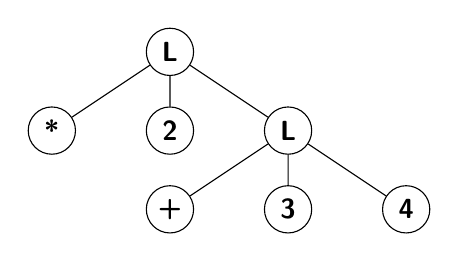
\begin{tikzpicture}[
            every node/.style={draw, circle,minimum size=0.6cm, inner sep=0pt,font=\sffamily\bfseries},
            level distance=1cm, ]
            \node {L} 
              child { node {*} }
              child { node {2} }
              child { node {L}
                child { node {+} }
                child { node {3} }
                child { node {4} }
              };
          \end{tikzpicture}
          \caption{N--arry syntax tree representing \texttt{(* 2 (+ 3 4))}}
          \label{fig:ast_example}
        \end{minipage}
        \hfill
        \begin{minipage}{0.48\textwidth}
          \centering
          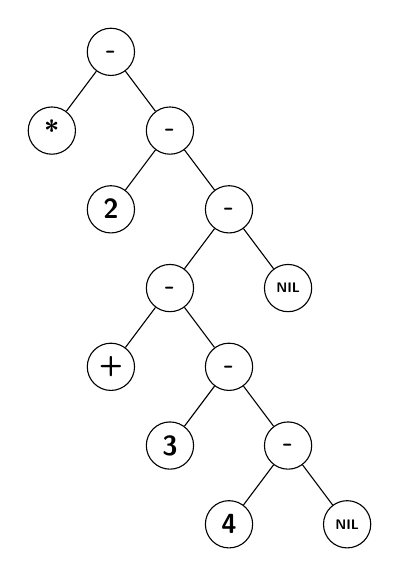
\begin{tikzpicture}[
            every node/.style={draw, circle, minimum size=0.6cm, inner sep=0pt, font=\sffamily\bfseries},
            level distance=1cm, ]
            \node {-}
              child { node {*} }
              child { node {-}
                child { node {2} }
                child { node {-} 
                  child { node {-} 
                    child { node {+} }
                    child { node {-}
                      child { node {3} }
                      child { node {-} 
                        child { node {4} }
                        child { node {\tiny{NIL}} } 
                      }
                    }
                  }
                  child { node {\tiny{NIL}} } 
                }
              };
          \end{tikzpicture}
          \caption{S--expression syntax tree representing\texttt{(* 2 (+ 3 4))}}
          \label{fig:ast_example2}
        \end{minipage}
      \end{figure}

      We will not discuss Stack based evaluation further as it would be hard to manage loops,
      unevaluated parts of the code and quite an overhead would be necessary to keep track of current operations.
      Essentially we would be building our own call stack and the solution would not be better than other options.

      Lisp is originally designed with s(symbolic)--expressions in mind as its internal structure and many of its functionalities are based on it.
      S--expression has some of its specific features. Since every list is essentailly 
      a~linked list, access time to its elements is $O(n)$ where $n$ is index if the elements. 
      The 'NIL' object used in Lisp also appears naturally in the s--expression as a list terminator, also usable as empty list. 
      Or for example a function \lstinline|CDR| returning the list without 
      the first element is straignhforward to implement as it is just the 'tail' node

      N--ary tree is more natural way to represent nested parenthesis structure
      \subsection{}

    


  \chapter{Implementation}
    \section{Architecture Overview}
    The interpreter is divided into several modules:
    \begin{itemize}
      \item \textbf{Preprocessor}: Removes comments and normalizes input (e.g., uppercase conversion).
      \item \textbf{Lexer}: Tokenizes input strings into meaningful tokens for parsing.
      \item \textbf{Parser}: Converts token arrays into an AST according to the defined grammar.
      \item \textbf{AST Module}: Provides functions for creating, copying, and freeing AST nodes.
      \item \textbf{Environment}: Manages variable storage and lookup.
      \item \textbf{Operators}: Implements built-in functions and arithmetic/logical operations.
      \item \textbf{REPL}: Handles user input, manages multi-line expressions, and invokes the interpreter.
    \end{itemize}

      % Example diagram using tikz
      \begin{figure}[h]
        \centering
        \begin{tikzpicture}
          \node (begin) [draw, rectangle] {Start};
          \node (preproc) [draw, rectangle, right=1.5cm of begin] {Preprocessor};
          \node (lexer) [draw, rectangle, right=1.5cm of preproc] {Lexer};
          \node (parse) [draw, rectangle, right=1.5cm of lexer] {Parser};
          \node (eval) [draw, rectangle, right=1.5cm of parse] {Evaluate};
          \draw[->] (begin) -- (preproc);
          \draw[->] (preproc) -- (lexer);
          \draw[->] (lexer) -- (parse);
          \draw[->] (parse) -- (eval);
        \end{tikzpicture}
        \caption{Interpreter workflow}
        \label{fig:workflow}
      \end{figure}
      \subsection{Used Data Dtructures}

    \section{Macros and Error handling}

    \section{Handling Input}
      \subsection{Arguments}
      \subsection{Repl}
    
    \section{Evaluation Pipeline}
      \subsection{Preprocessor}
      \subsection{Lexer}
      \subsection{Parser}
      \subsection{Evaluation}
        \subsubsection{Environment}
        \subsubsection{Operators}

    \section{Memory Management}

  \chapter{User guide}
  \chapter{conclusion}
  \iffullbuild
    \appendix{}
    \chapter{}
    \label{assignment}
    \includepdf[pages=-]{sw2025-02.pdf}
  \fi
\end{document}